% ---
% Capa
% ---
\imprimircapa
% ---

% ---
% Folha de rosto
% (o * indica que haverá a ficha bibliográfica)
% ---
\imprimirfolhaderosto*
% ---

% ---
% Inserir a ficha bibliografica
% ---
% http://ficha.bu.ufsc.br/
\begin{fichacatalografica}
	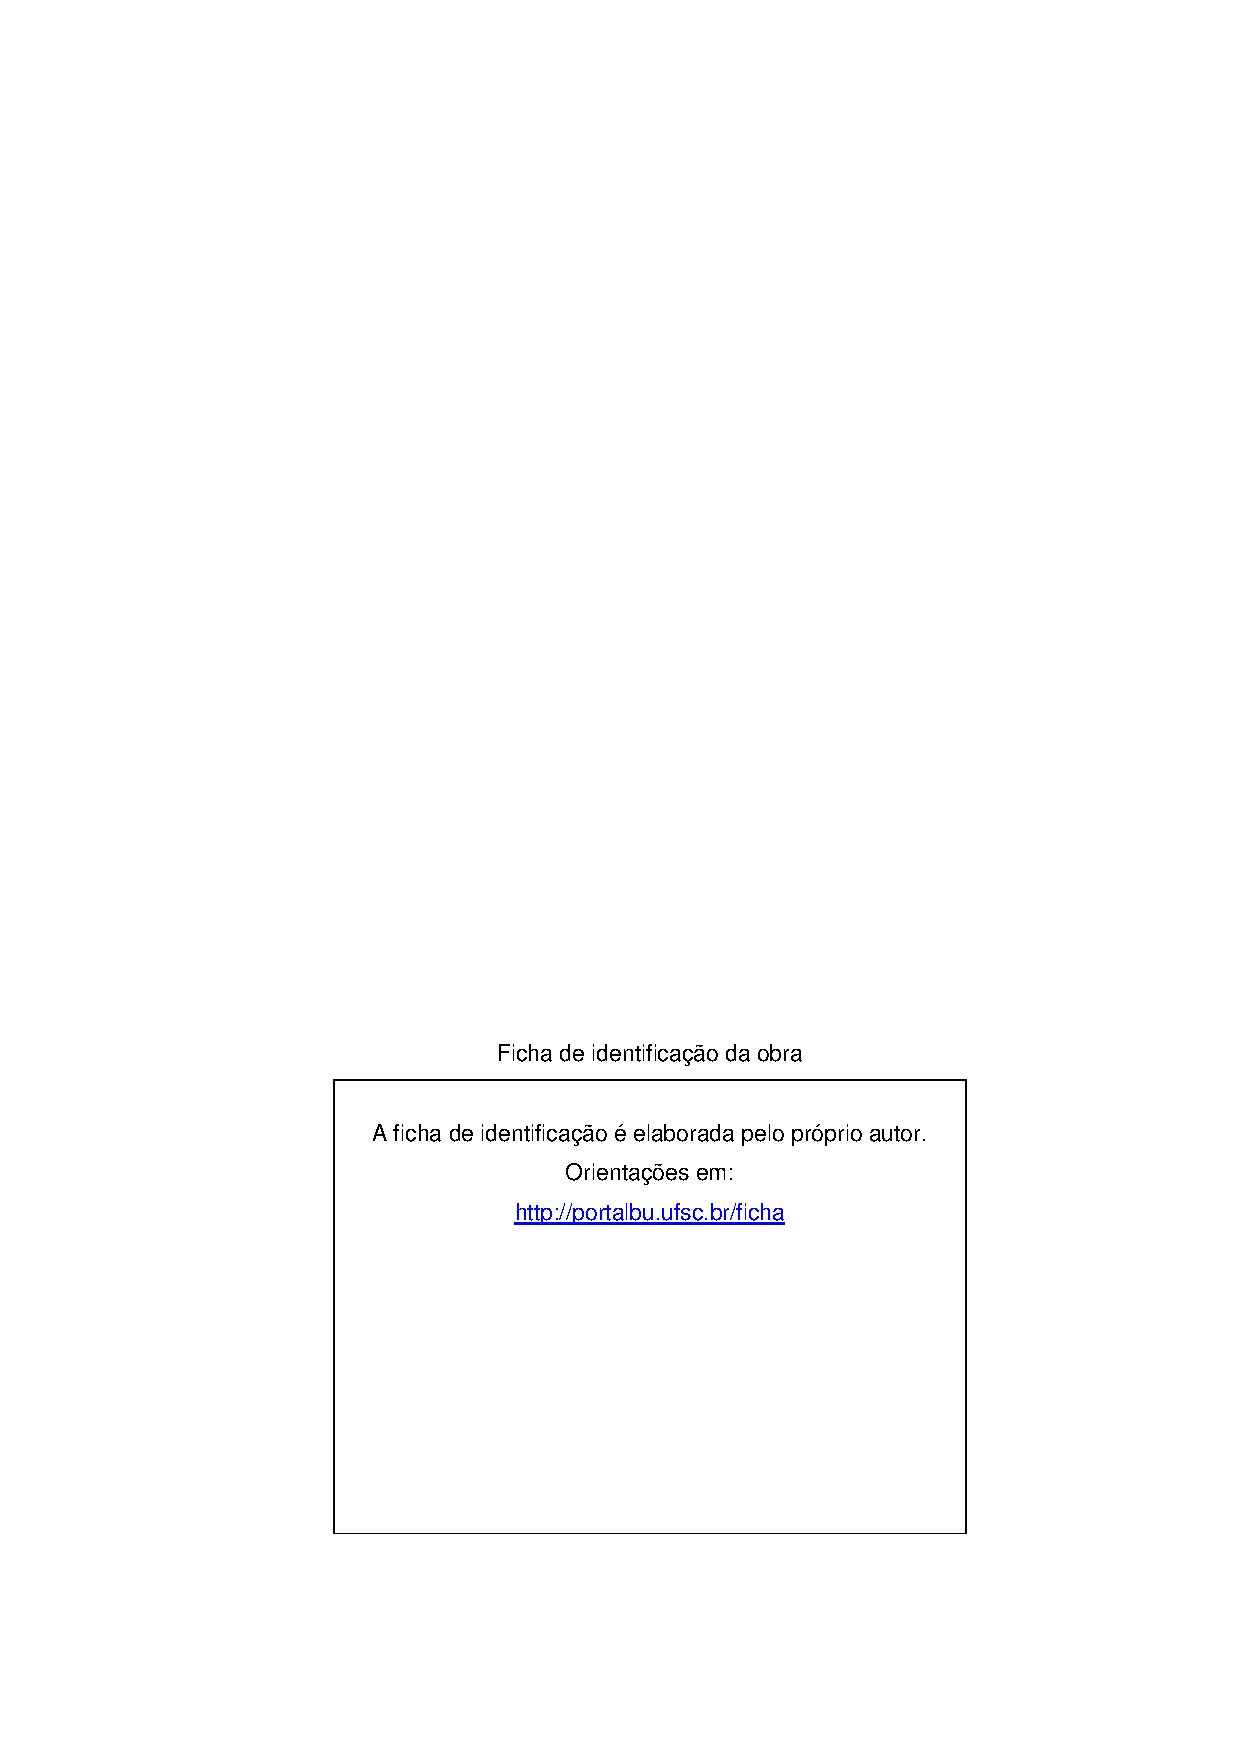
\includepdf{beforetext/Ficha_Catalografica.pdf}
\end{fichacatalografica}
% ---

% ---
% Inserir folha de aprovação
% ---
\begin{folhadeaprovacao}
	\OnehalfSpacing
	\centering
	\imprimirautor\\%
	\vspace*{10pt}		
	\textbf{\imprimirtitulo}%
	\ifnotempty{\imprimirsubtitulo}{:~\imprimirsubtitulo}\\%
	%		\vspace*{31.5pt}%3\baselineskip
	\vspace*{\baselineskip}
	%\begin{minipage}{\textwidth}
	% ~do~\imprimirprograma~do~\imprimircentro~da~\imprimirinstituicao~para~a~obtenção~do~título~de~\imprimirformacao.
	Este~\imprimirtipotrabalho~foi julgado adequado para obtenção do Título de “\imprimirformacao” e aprovado em sua forma final pelo~\imprimirprograma. \\
		\vspace*{\baselineskip}
	\imprimirlocal, \imprimirdata. \\
	\vspace*{2\baselineskip}
	\assinatura{\OnehalfSpacing\imprimircoordenador \\ \imprimircoordenadorRotulo~do Curso}
	\vspace*{2\baselineskip}
	\textbf{Banca Examinadora:} \\
	\vspace*{\baselineskip}
	\assinatura{\OnehalfSpacing\imprimirorientador \\ \imprimirorientadorRotulo}
	%\end{minipage}%
	\vspace*{\baselineskip}
	\assinatura{Prof.(a) Sergio Yesid Gomez, Dr(a).\\
	Avaliador(a) \\
	Departamento de Engenharia Química (EQA/UFSC)}

	\vspace*{\baselineskip}
	\assinatura{Cristine Carraro, Dr(a).\\
	Avaliador(a) \\
	Departamento de Engenharia Mecânica e Materiais (EMC/UFSC)}


\end{folhadeaprovacao}
% ---

% ---
% Dedicatória
% ---
% \begin{dedicatoria}
% 	\vspace*{\fill}
% 	\noindent
% 	\begin{adjustwidth*}{}{5.5cm}     
% 		Este trabalho é dedicado aos meus colegas de classe e aos meus queridos pais.
% 	\end{adjustwidth*}
% \end{dedicatoria}
% ---

% ---
% Agradecimentos
% ---
\begin{agradecimentos}
	Aos meus pais, Sivaldo Leite e Verônica Boimer, por todo suporte e incentivo ao longo da minha formação, provendo mais do que o necessário para me dar uma educação de qualidade.

	À Tayná Moraes, pela companhia nos momentos mais difíceis e mais felizes, por acreditar em mim e na ideia do trabalho.

	Aos amigos que fiz em sala de aula e em laboratórios, em especial no LINDEN, pois tornaram todo processo mais divertido, interessante e enriquecedor.

	Ao Dachamir Hotza, por ser uma pessoa acolhedora, atenciosa e um orientador exemplar, por todas orientações e oportunidades, não apenas durante o trabalho, mas ao longo de todo o curso.

	À UFSC, por ser uma instituição que abraça a diversidade e dá suporte à formação de pessoas conscientes e preocupadas com a sociedade e o planeta.


\end{agradecimentos}
% ---

% ---
% Epígrafe
% ---
\begin{epigrafe}
	\vspace*{\fill}
	\begin{flushright}
		\textit{``Nunca duvide que um pequeno grupo de pessoas conscientes e engajadas possa mudar o mundo.\\
			De fato, foi sempre assim que o mundo mudou.\\
			(Margaret Mead)}
	\end{flushright}
\end{epigrafe}
% ---

% ---
% RESUMOS
% ---

% resumo em português
\setlength{\absparsep}{18pt} % ajusta o espaçamento dos parágrafos do resumo
\begin{resumo}
	\SingleSpacing

	A Política Nacional de Resíduos Sólidos (PNRS), criada pela Lei 12.305 de 12
	de Fevereiro de 2010, dispõe uma série de diretrizes relacionadas à gestão de resíduos sólidos. A partir disso, ferramentas que permitam a captação de dados sobre todas as etapas do descarte de resíduos vêm sido criadas, um exemplo disso é o Manifesto de Transporte de Resíduos (MTR), documento para rastreabilidade dos resíduos a ser preenchido por todos englobados dentro do Plano de Gerenciamento de Resíduos Sólidos (PGRS), disponível digitalmente a nível nacional. Este instrumento tem também o pretexto de servir como uma base de dados mais completa e unificada sobre a geração, armazenamento, transporte e destinação de resíduos no Brasil. Assim, as informações contidas no MTR podem ser valiosas, abrindo oportunidade para a movimentação de uma economia de aproveitamento de resíduos. Com esse intuito, o presente trabalho propõe a criação de um aplicativo web reunindo os dados de MTR a fim de conectar geradores a potenciais consumidores de resíduos no âmbito industrial em Santa Catarina (SC). Estudam-se os conceitos para tal sistema, faz-se o tratamento e análise dos dados de MTR e desenvolve-se um protótipo de aplicação.
	
	\textbf{Palavras-chave}: Manifesto de Transporte de Resíduos (MTR). Redirecionamento de resíduos sólidos. Aplicação Web.
\end{resumo}

% resumo em inglês
\begin{resumo}[Abstract]
	\SingleSpacing
	\begin{otherlanguage*}{english}

		The National Solid Waste Policy (PNRS), created by Law 12.305 on February 12, 2010, establishes a series of guidelines related to the management of solid waste. After this, tools that allow the collection of data on all stages of waste disposal have been created, an example of which is the Waste Transport Manifest (MTR), a document for the traceability of waste to be filled out by all those included in the Solid Waste Management Plan (PGRS), it is digitally available nationwide. This instrument also aims to serve as a more comprehensive and unified database on the generation, storage, transport, and disposal of waste in Brazil. Thus, the information contained in the MTR can be valuable, opening up opportunities for the development of a waste recovery economy. With this intention, the present work proposes the creation of a web application gathering MTR data to connect generators to potential consumers of waste in the industrial field in Santa Catarina (SC). Concepts for such a system are studied, and the treatment and analysis of MTR data are carried out, leading then to the development of a prototype application.
		
		\textbf{Keywords}: Waste Transport Manifest (MTR). Waste redirection. Web application.
	\end{otherlanguage*}
\end{resumo}

%% resumo em francês 
%\begin{resumo}[Résumé]
% \begin{otherlanguage*}{french}
%    Il s'agit d'un résumé en français.
% 
%   \textbf{Mots-clés}: latex. abntex. publication de textes.
% \end{otherlanguage*}
%\end{resumo}
%
%% resumo em espanhol
%\begin{resumo}[Resumen]
% \begin{otherlanguage*}{spanish}
%   Este es el resumen en español.
%  
%   \textbf{Palabras clave}: latex. abntex. publicación de textos.
% \end{otherlanguage*}
%\end{resumo}
%% ---

{%hidelinks
	\hypersetup{hidelinks}
	% ---
	% inserir lista de ilustrações
	% ---
	\pdfbookmark[0]{\listfigurename}{lof}
	\listoffigures*
	\cleardoublepage
	% ---
	
	% ---
	% inserir lista de quadros
	% ---
	\pdfbookmark[0]{\listofquadrosname}{loq}
	\listofquadros*
	\cleardoublepage
	% ---
	
	% ---
	% inserir lista de tabelas
	% ---
	\pdfbookmark[0]{\listtablename}{lot}
	\listoftables*
	\cleardoublepage
	% ---
	
	% ---
	% inserir lista de abreviaturas e siglas (devem ser declarados no preambulo)
	% ---
	\imprimirlistadesiglas
	% ---
	
	% ---
	% inserir lista de símbolos (devem ser declarados no preambulo)
	% ---
	\imprimirlistadesimbolos
	% ---
	
	% ---
	% inserir o sumario
	% ---
	\pdfbookmark[0]{\contentsname}{toc}
	\tableofcontents*
	\cleardoublepage
	
}%hidelinks
% ---